\section{Design description}
This section describes the design of the DSL implemented by AiryScript. It
contains information on both its development process and its current syntax. The
next section,
\begin{itemize}
  \item Section \ref{sec:devising_syntax} describes the syntax of the
    predecessors of AiryScript, and their influence on its current syntax.
%
  \item Section \ref{sec:syntax_spec} describes the general syntax of AiryScript
    for describing data and describing data structures through types.
%
  \item Section \ref{sec:structural_type_system} goes into some more detail
    describing the structural type system of AiryScript.
%
  \item Section \ref{sec:operations_spec} describes the general syntax of
    AiryScript for describing and calling operations.
%
  \item Section \ref{sec:protecting} explains why AiryScript provides the user
    with operations that are sometimes more powerful than they need to be.
\end{itemize}

\noindent
Section \ref{sec:operations} thoroughly documents all of the operations that
AiryScript offers, using the syntax provided in Section \ref{sec:syntax_spec}
and Section \ref{sec:operations_spec}.

\subsection{Devising a language syntax}
\label{sec:devising_syntax}
This section documents how the development process of the syntax of AiryScript.

AiryScript is roughly the third fairly complete language we came up with during
development, and contains elements of both the first and the second language. In
the following subsections, we discuss these ‘iterations’ chronologically.

\subsubsection{Iteration one}
In a first serious attempt at defining AiryScript we tried to approximate
natural language as closely as possible.

The following commands are examples of expressions in this language.
\begin{lstlisting}[language=empty,frame=single]
ADD CITY Brussels, Edinburgh
ADD AIRPORT Brussels TO Brussels, Edinburgh TO Edinburgh
ADD COMPANY SAB
ADD SEATTYPE Economy, Business, First class
ADD AIRPLANE Boeing 007 WITH 100 Economy SEATS, 20 Business SEATS
ADD TIME Brussels TO Edinburgh 1h22 BY Boeing 007
ADD TEMPLATE SAB888 FROM Brussels TO Edinburgh BY Boeing 007
    WITH 21 euro FOR Economy SEATS, 34 euro FOR Business SEATS
        FROM 15/12/2012 TO 9/01/2014
    WITH 168 euro FOR Economy SEATS, 370 euro FOR Business SEATS
        FROM 15/06/2015 TO 9/12/2016, EACH 2nd FRIDAY OF THE MONTH
\end{lstlisting}

We decided to get rid of this language because of the following reasons.
\begin{itemize}
  \item The ‘natural language’ in our DSL is really quite different from real
    natural language. We decided that it is not possible to make complicated
    commands like adding a template look like natural language, because no
    person would try to specify all there is to know about a template in a
    single sentence.
  \item Natural language is different for different persons. The code above
    is easy to understand, but when trying to document or write a statement in
    it it quickly becomes clear that this language, like natural language, is
    fairly irregular and inconsistent.
  \item Irregular languages are difficult to learn.
  \item Writing a parser for this language is difficult, both because it is
    irregular and because of the syntax itself. We prefer not to have any need
    for semicolons or impose indentation rules on our users, which is pretty
    much impossible using this syntax, which uses no commas, parenthesis or
    quotation marks to separate values from language keywords.
\end{itemize}
Some of the things we learned in this process are the following.
\begin{itemize}
  \item When designing a language, one has to focus on the more complicated
    statements that language should be capable of expressing.

    Most of the languages one can come up with look nice when expressing the
    creation of a city, but almost none of them are capable of describing
    templates without turning ugly.
  \item It is a bad idea to
  try and make the language look like natural language.
  \item It is probably a good idea to keep in mind that the DSL needs to be
    machine-readable.
  \item Some things are just way more complicated than people ever care to think
    about. Statements like ‘a flight flies every year at 12h during every second
    Friday of the months August and November’ are very powerful and difficult to
    express in a consistent manner, store and search. Implementing an efficient
    system that is capable of handling periods like this are not in the scope of
    this assignment.
\end{itemize}


\subsubsection{Iteration two}
In a second attempt at defining the AiryScript syntax we came up with a very
general, powerful and compact syntax that is most certainly targeted towards
users with other backgrounds than the language of iteration one.

The following commands are examples of expressions in this language. They have
the same effect as the code in iteration one, except from the fact that we got
rid of the ‘second Friday of the month’-statement.
\begin{lstlisting}[language=empty,frame=single]
AIRPORT { name: Edinburg, city: { name : Edinburg } }
AIRPORT { name: Zaventem, city: { name : Brussels } }
TEMPLATE {
  fln: SAB888
  from: (name: Brussels)
  to: (name: Edinburgh)
  type: { name: "Boeing 007" }
  periods: [
    { from: 15/12/2012, to: 9/01/2014, prices: [
        {type: {name: economy}, price: {euro: 21}},
        {type: {name: business}, price: {euro: 34}}
    ]},{ from: 15/06/2015, to: 9/12/2016, prices: [
        {type: (name: economy), price: {euro: 268}},
        {type: (name: business), price: {euro: 370}}
    ]}
  ]
}
\end{lstlisting}
We envisioned this to be a strongly, statically typed language that did not
require the user to ever really specify any types. Curly brackets create a new
structure that would automatically be added to the database, whereas parenthesis
select a structure that already exists. We also developed a syntax to modify
existing structures.

We decided to get rid of this language because of the following reasons.
\begin{itemize}
  \item Complicated statements can become quite difficult to read, especially
    for people who are not familiar with the types behind the language.
  \item Although a language shouldn’t be based on natural language like in
    iteration one, it is always good to be able to read out loud what a series
    of statements does. We cannot do that in this language.
  \item This language is heavily inspired by the structure of our problem
    domain, and forces its users to also be aware of this structure.
  \item The syntax of this language is very general. Without changing too much,
    it could replace SQL for most queries, not just for our database structure
    but for any database structure. This is not a good sign: GlobAir Inc.  is
    dissatisfied with SQL, and wants us to create a \emph{different}
    language.
  \item Because queries can be nested indefinitely and statements have to have
    access to information that is available on a higher level\footnote{For
      example, to define a period we have need of a template to bind it to. In
      the example, we do not specify the FLN of the periods we create, which
      automatically assigns the FLN of the template we are creating on a higher
      level to it.},
    implementing this language would be very hard.
\end{itemize}
Some of the things we learned in this process are the following.
\begin{itemize}
  \item Consistency is important, but so is readability. The language in
    iteration one focussed too much on readability, the language in iteration
    two focussed too much on consistency.
  \item We should try to forget about the database and problem domain structure,
    and try to look trough the eyes of the user of our DSL.
  \item We are dealing with a DSL; we should not be shy about introducing
    language features and syntax that is only relevant for the specific problem
    domain of AiryScript.
\end{itemize}

\subsubsection{Iteration three}
The syntax of the third iteration is the final syntax of AiryScript. The next
sections therefore discuss this syntax into full detail. This section provides a
sneak-peak of what the syntax of AiryScript looks like.

The following commands have the same effect as the code shown for iteration two.
\begin{lstlisting}[language=airyscript,frame=single]
  ADD CITY {name : Brussels}
  ADD CITY {name : Edinburgh}
  ADD AIRLINE {fln: Sab, name: Sabena}
  ADD SEAT TYPE {economy}
  ADD SEAT TYPE {business}
  ADD SEAT TYPE {"first class"}
  ADD AIRPLANE TYPE {
      name: "Boeing 007"
  } WITH SEATS [
      {type: economy, amt: 100},
      {type: business, amt: 20}
  ]
  ADD TEMPLATE {
      fln: SAB888,
      from: {name: Brussels},
      to: {name: Edinburh},
      airplaneType: {name: "Boeing 007"},
  } WITH SEAT INSTANCES [
      {type: economy, price: {dollar: 21}},
      {type: business, price: {dollar: 34}}
  ] AND WITH PERIODS [
      {
          from: {d: 25, m: 12, y: 2012},
          to: {d: 9, m: 1, y: 2014},
          departure: {h :12}
      },{
          from: {d: 15, m:  6, y: 2012},
          to: {d: 9, m: 12, y: 2016},
          departure: {h: 15, m:35}
      }
  ]
  CHANGE SEAT INSTANCES OF FLIGHT {
      template: {fln: SAB888},
      during: {
          from: { d: 15, m:  6, y: 2012 },
          to: { d: 9, m: 12, y: 2016 },
      }
  } TO [
    {type: business, price: {dollar: 268}},
    {type: economy, price: {dollar: 370}}
  ]
\end{lstlisting}
We believe this language is a healthy mix between elements from the languages in
iteration one and two.
\begin{itemize}
  \item It is possible to read sentences out loud, just like in the language of
    iteration one. The labels and commands in front of structures make them
    quite readable.

    We believe that even without ever having seen a description of what the
    different operations in our language do or having seen a
    description of the syntax of our language, people familiar with the domain
    of Section \ref{sec:domain} are capable of understanding what the code above
    does.
  \item The language is consistent, just like in iteration two. When provided
    with the manual, users should quickly be able to start writing queries.
  \item The language is quite robust. Lots of invalid queries produce parsing
    errors.
  \item Unlike the languages in iteration one and two, this language can be
    implemented!
\end{itemize}
Note that this is actually a very bad example to show off the new syntax.  The
old syntaxes still assumed a domain model where prices are linked to time
periods. This new syntax uses the domain model that Section \ref{sec:domain}
describes, and links prices to a template. We can still achieve the same pricing
configuration by changing the prices of the flights over a specified time
period, but this requires an additional operation.


\subsection{Protecting the user}
\label{sec:protecting}
Before we continue with the technical details of the meta model of our DSL
that we choose after the last iteration we take a small sidestep.

This section explains our decision to prefer more powerful operations over more
safe ones. We use the ‘change city’ operation as a simple example where the
difference between powerful and safe is clearly visible.

At some point in the design of the DSL, we have to decide on specific types and
operations. For changing distances, we can come up with two possibilities that
make perfect sense.

\begin{center}
\begin{tabular}{p{0.5\textwidth}p{0.5\textwidth}}
  Approach one & Approach two \\\hline
  \begin{lstlisting}
Dist = {
    ?from:Airport,
    ?to: Airport,
    ?dist:Int
}
Dist_data = {
    from:Airport,
    to: Airport,
    dist:Int
}

CHANGE DISTANCE <Dist> TO <Dist>
  \end{lstlisting} &
  \begin{lstlisting}
Dist = {
    from:Airport,
    to: Airport
}
Dist_data = {
    from:Airport,
    to: Airport,
    dist:Int
}


CHANGE DISTANCE <Dist> TO <Int>
  \end{lstlisting}
\end{tabular}
\end{center}
The language syntax is expressive enough to be able to handle both approaches,
but naturally we have to decide on only one.

\paragraph{Approach one}
defines a very general change operator that not only allows
changing the distance of a single pair of airport, but also the \tye{from} and
\tye{to} properties of existing pairs of airports or even groups of pairs of
airports.

The main advantage of this approach lies it its consistency.  We can use very
similar operation definitions for changes to other types of data, for example
\begin{quote}
  \tye{CHANGE FLIGHTTIME <FlightTime> TO <FlightTime>}
\end{quote}
and
\begin{quote}
  \tye{CHANGE TEMPLATE <Template> TO <Template>}
  ,
\end{quote}
which really means that we have a generic change operations.

This is just a single example, but taking into consideration all types we can
distinguish the following advantages and disadvantages.
\begin{itemize}
  \item The advantage of this approach is that we have fairly few, simple
    operations that are easy for users to learn. There is also the possibility
    to execute very powerful queries.
  \item The disadvantage of this approach is that it allows users to write
    queries that are \emph{too} general. It allows users to execute
    operations that do not make sense.
\end{itemize}

\paragraph{Approach two}
defines a more restricted change distance operator that only allows changing
single, existing distances between pairs of cities.

Approach one allows users to execute queries like
\begin{quote}
  \tye{CHANGE DISTANCE {from: {name: Zaventem}} TO {dist: 1000}}
\end{quote}
or even
\begin{quote}
  \tye{CHANGE DISTANCE {dist: 5000} TO {dist: 1000}}
  .
\end{quote}
The first query changes the distance of all flights that start from the Zaventem
airport to 1000km, which of course only make sense as long as there is only one
such distance in the database. The second query changes the distance between all
pairs of cities with a distance of 5000km to a distance of 1000km. The main
advantage of the second approach is therefore increased safety.

These are just examples, but taking into consideration all types we can
distinguish the following advantages and disadvantages.
\begin{itemize}
  \item The advantage of this approach is increased safety for the users, as
    they are no longer capable of destroying the contents of the database with a
    single query.
  \item The disadvantage of this approach is increased language complexity
    for manipulating more complicated domain elements. We potentially
    have to create a lot of different selection types and operations for the
    different things we want to be able to change about these elements.

    Also, queries become less powerful. It is probably impossible to restrict
    users so much that he cannot do anything wrong without imposing some
    restrictions that are usually just irritating. For example, approach one
    does not allow a user to rectify his or her mistake after entering a distance
    between York Airport and Zaventem instead of New York and Zaventem: he has
    to delete the mistake and add a new distance again. As another example,
    allowing the user to specify prices for only a single flight at a time makes
    the ‘change prices’ operation safer, but also less powerful.
\end{itemize}

\paragraph{Our train of thought}
While in the case of airports it is fairly easy to protect users from themselves
by not allowing them to execute non-sensible queries, this is not the case for
more complicated domain elements like flights or flight templates. We feel that
if take approach two here, then this means that we take it upon ourselves to
protect users from themselves like this for all types and operations, also the
more complicated ones.

Because we saw that the number of types and operations that are necessary to
prevent users from executing potentially disastrous queries on the database
(approach two) is much greater than the number of types and operations necessary
for approach one, we decided to take approach one for AiryScript. We think that
this is usually something you have discuss with the client of the DSL. Which
approach is best also heavily depends on the background of the users of
AiryScript.

\paragraph{AiryScript is still safer than SQL}
While we give users access to powerful operations and do not protect them from
filling up the database with nonsense, AiryScript certainly does aim to make it
impossible for users to make data \emph{inconsistent}. This is the only
requirement specified in the assignment. For example, it is impossible to create
a template where an airplane type $t$ flies from city $a$ to city $b$ if there
is no flight time available for the combination of $a$, $b$ and $t$. It is also
impossible to delete a flight time for $a$, $b$, $t$ as long as there still
exists a template that relies on it. Basically, AiryScript makes sure all the
constraints specified in the domain of Section \ref{sec:domain} are kept.


\subsection{The semantic model}

\begin{figure}
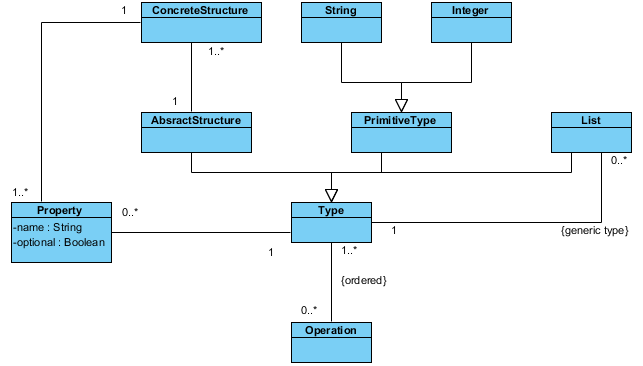
\includegraphics[width=\textwidth]{img/semanticModel.jpg}
\caption{High level semantic model.}
\label{fig:semantic-model}
\end{figure}

Lets look at how the final structure of our language looks like after the
third iteration. This is represented schematically in \ref{fig:semantic-model}.
This is the high level semantic model of our DSL, we did not include all the
individual operations and structure types in the diagram but they all satisfy
the given model.

The semantic model is basically the point of contact between the parser and
the handler (the part of the system executing those operations, which involves
querying the database). The parser will populate this model, while the handler
will act upon this model, which is a nice way of decoupling these 2
functionalities.

Concretely all the operations and structures in this semantic model map 1 to 1
with scala case classes. The parser will parse a string into the proper
\class{Operation}-case class. This piece of data can be passed to the handler to
actually perform the operation.

But we are running ahead, lets first examine these operations, structures and
primitive types in more detail.


\subsection{Describing and creating structures}
\label{sec:syntax_spec}
This section specifies how to create structures in AiryScript and explains the
notation that Section \ref{sec:operations} uses to specify types. Even though
AiryScript does not require its users to declare types or provide them with
the possibility to define their own types, knowing how to describe types and how
the typing system of AiryScript works is important, since AiryScript is a typed
language.

\paragraph{Primitive types}
AiryScript supports strings and integers as primitive types. The statements
\begin{quote}
  \tye{5}\\
  \tye{502349}
\end{quote}
define the integers 5 and 502349. The statements
\begin{quote}
  \tye{IAmFreeOfSpacesAndIThereforeDoNotRequireQuotation}\\
  \tye{"I am not free of spaces and therefore I do require quotation"}\\
  \tye{"IAmFreeOfSpacesYetICanStillUseQuotation"}
\end{quote}
each define a string. Users should surround strings that contain spaces and/or
commas with quotation marks.


\paragraph{Structures}
AiryScript also supports structures. Structures consist of one or several
properties. Properties have a name and a value. A name is always a string that
does not contain any spaces. A value is either a primitive value or another
structure. Names are separated from values by a colon, properties are separated
from each other by commas and structures are defined within curly brackets. As
an example,
\begin{quote}
  \ins{a: 10, b: 5}
\end{quote}
defines a structure with a property named \tye{a} that has an integer primitive
value of ten and a property named \tye{b} that has an integer primitive value of
five. AiryScript is not sensitive to whitespace or newlines. For example,
\begin{quote}
  \begin{verbatim}
{  a:10, b       :
                    5}
  \end{verbatim}
\end{quote}
defines the same structure as before.


\paragraph{Basic structure types}
In the documentation,
\begin{quote}
  \ty{A}\tye{ = \ins{a: Int, b: String}}
\end{quote}
defines \ty{A} to be shorthand for the type that collects all structures that
have properties named \tye{a} and \tye{b} with respective types \tye{Int} and
\tye{String}. Structures that define an \tye{Int} and a \tye{String} with
different names do not belong to type \ty{A}. This simple definition completely
describes a type. If AiryScript would allow users to define their own types and
operations, this would be the syntax it would use.

As an example, the following two lines each define a structure that is an
instance of \ty{A}.
\begin{quote}
  \ins{a: 10, b: tomatoes}\\
  \ins{b: "bottles of beer", a: 10}\\
\end{quote}


\paragraph{Types with optional properties}
In the documentation,
\begin{quote}
  \ty{B}\tye{ = \ins{a: Int, ?b: Int, ?c: String}}
\end{quote}
defines \ty{B} to be shorthand to the type that collects all structures that
have properties named \tye{a} with type \ty{Int}, and that optionally has two
more properties with names \tye{b} and \tye{c} and values with respective types
\ty{Int} and \ty{String}. Structures that either have parameters
with names different from \tye{a}, \tye{b} or \tye{c} or that have an \tye{a},
\tye{b} or \tye{c} with a different type do not belong to \ty{B}.

As an example, all of the following lines define a structure that is an
instance of \ty{B}.
\begin{quote}
  \ins{c: "bottles of beer", a: 10}\\
  \ins{a: 10, b: 5 c: "bottles of beer"}\\
  \ins{a: 10, b: 5}
\end{quote}

\paragraph{Types of nested structures}
In the documentation,
\begin{quote}
  \ty{C}\tye{ = \ins{a: B, b: String}}
\end{quote}
defines \ty{C} to be shorthand for the type of structures that have properties
with names \tye{aB} and \tye{aString}, with types \tye{B} and \tye{String}
respectively. Since we can further expand \ty{B}, this is in turn shorthand for
\begin{quote}
  \ins{a: \ins{a: Int, ?b: Int, ?c: String}, b: String}.
\end{quote}

As an example, the following line defines a structure that is an instance of
\ty{C}.
\begin{quote}
  \ins{b: \ins{a: 10, b: 5}, a: "bottles of beer"}
\end{quote}

\paragraph{Union types}
In the documentation,
\begin{quote}
  \ty{D}\tye{ = A | B}
\end{quote}
defines a type that contains both the structures contained in \tye{A} and the
structures contained in \tye{B}.

As an example, both of the following lines define a structure that is an
instance of \ty{D}.
\begin{quote}
  \ins{a: 10, b: tomatoes}\\
  \ins{a: 10, b: 5}
\end{quote}


\paragraph{Lists}
In the documentation,
\begin{quote}
  \ty{E}\tye{ = [Int]}
\end{quote}
defines a type that contains a list of integers. List elements are separated
by commas and defined within square brackets. Naturally, lists can also occur
within structures. The ordering of elements in a list is preserved during
interpretation; whether or not the ordering matters depends on the operation the
list is passed to.

As an example, the following two lines each define an instance of \ty{E}.
\begin{quote}
  \tye{[1,2,3,4]}\\
  \tye{[   5 , 2,1,2]}
\end{quote}


\subsection{Type system}
\label{sec:structural_type_system}
This section describes the type system of AiryScript. Section
\ref{sec:type_classification} classifies the type system into some categories
that are well-known in computer science. Section \ref{sec:type_example} provides
some examples to illustrate how the type system works.

\subsubsection{Classification}
\label{sec:type_classification}
The type system of AiryScript is.
\begin{description}
  \item[Strongly typed] When AiryScript expects a parameter of type $T$, it is
    not possible to provide it with another type. It is not possible to cast
    values to another type, and there is no type that matches all types.
  \item[Statically typed] AiryScript determines and checks types while parsing.
  \item[Structural] Type compatibility and equivalence are determined by the
    type’s actual structure or definition. Subtyping relations cannot be
    declared explicitly but are created automatically by shared structure.
  \item[Implicit] AiryScript never requires the user to explicitly declare any
    types.
\end{description}

\subsubsection{Examples}
\label{sec:type_examples}
This section discusses the structural type system of AiryScript by providing an
extended example.

We look at the type of object $o$ defined as
\begin{quote}
  \ins{a: 10, c: "bottles of beer"}.
\end{quote}
The type of $o$ is \ins{a: Int, c: String}. A discussion of the relation between
the type of $o$ and the following types should clarify how the type system of
AiryScript works.
\begin{quote}
  \ty{A}\tye{ = \ins{c: String, a: Int}}\\
  \ty{B}\tye{ = \ins{a: Int, ?b: Int, ?c: String}}\\
  \ty{C}\tye{ = \ins{a: Int, b: String, c: String}}\\
  \ty{D}\tye{ = \ins{c: Int, a: String}}
\end{quote}
\begin{itemize}
  \item $o$ is an instance of \ty{A}. In fact, \ty{A} is just shorthand for
    $o$’s type. The order in which \tye{c} and \tye{a} appear does not matter:
    as far as AiryScript is concerned the types \ins{c: String, a:Int}
    and \ins{a:Int, c: String} are identical. The one-dimensional nature of text
    makes it so that we have to specify an ordering that is actually
    meaningless.

  \item $o$ is an instance of \ty{B}, which also means that \ty{A} is a subtype
    of \ty{B}.  We can ‘ignore’ the optional properties of \tye{c}. Note that
    the fact that \ty{C} can be a super type of \ty{B} without having to specify
    this in \ty{C} is quite special, and typical for structural type systems.

  \item $o$ is not an instance of \ty{C}. \ty{A} and \ty{C} are not related.

    While in most existing structural type systems, like the one of Haxe, \ty{C}
    would be a subtype of \ty{B}, this is not the case in AiryScript. This is
    because AiryScript does not allow users to specify properties that are not
    defined by the type. \ins{a: "bla"} is not an instance of type \ins{a:
    String, b: String} in AiryScript. The only way to to create a typing
    hierarchy is through optional parameters.

  \item $o$ is not an instance of \ty{D}. \ty{A} and \ty{D} are not related.

    Even though \ty{D} also consists of two properties, one an \tye{Int} and one
    a \tye{String}, \ty{D} is unrelated to \ty{A} because the names of these
    properties are different in \ty{D} and \ty{A}. The names of properties are
    part of the type, which allows AiryScript to make types independent of the
    order of their properties.
\end{itemize}

\subsection{Describing and calling operations}
\label{sec:operations_spec}
This section specifies how to perform operations in AiryScript and explains the
notation that Section \ref{sec:operations} uses to specify operations.


\paragraph{Basic operations}
In the documentation,
\begin{quote}
  \tye{DO INTEGER <Int>}
\end{quote}
specifies an operation that takes an integer. Together with the operation
signature, the documentation defines what an operation does. Users can call the
function above in an AiryScript script file as
\begin{quote}
  \tye{DO INTEGER 5}
  .
\end{quote}
It is also possible to write
\begin{quote}
  \tye{DO INTEGER \{5\}}
  ;
\end{quote}
we leave it up to the user to decide which syntax he/she likes best.
Of course, operations can also take structures as their arguments. Users can
separate all parts by one or multiple spaces and/or newlines. For example,
\begin{quote}
\begin{verbatim}
DO          INTEGER
      5 DO INTEGER 10
\end{verbatim}
\end{quote}
does what the user wants and performs the operation \tye{DO INTEGER} twice.
Note that AiryScript does not require the user to put a semicolon at the end of
an operation or between operations.
AiryScript does not parse input like
\begin{quote}
  \tye{ADDINTEGERS 5 10} .
\end{quote}

\paragraph{Separated operations}
Some operations in AiryScript take multiple arguments. Although AiryScript is
capable of parsing input like
\begin{quote}
  \tye{DO STUFF TO DURING <Stuff> <Something> <Period>}
  ,
\end{quote}
we believe this is not very legible. AiryScript’s operations are therefore
usually split up like
\begin{quote}
  \tye{DO <Stuff> TO <Something> DURING <Period>}
\end{quote}
to increase legibility. Note that this really does define a \emph{single
operation} that has access to three arguments (instances of \tye{Stuff},
\tye{Something} and \tye{Period}) and not three operations (\tye{DO}, \tye{TO}
and \tye{DURING}) that each operate on a single argument.

The order of the keywords is fixed, so users are not able to write
\begin{quote}
  \tye{DO \{…\} DURING \{…\} TO \{…\}}
  .
\end{quote}

AiryScript allows users to put spaces and newlines in between keywords, but we
advise users to write legible code by keeping these kind of ‘separated
operations’ together, and not separate them by newlines.


%Operations in AiryScript are always capitalized.




%\subsection{Though decisions}
%\label{sec:though_decisions}
%This section documents some of the tougher choices we had to make when designing
%specific operations for the language.
%
%This section often refers to actual operations in the language, but is not a
%language description. See Section \ref{sec:operations} for a consistent and
%complete overview of all operations and types.
%
%As is often the case with though choices, each possible decision has advantages
%and disadvantages. We made choices only after several hours of discussion.




\section{Types and operations}
\label{sec:operations}

In this section we will give a detailed overview of all the available
operations and types in the concrete syntax of our DSL.

% \subsection{Relation with the semantic-model}
% 
% Before we do this however we want to relate these operations to our
% \class{Operations}s from the semantic model (\ref{fig:semantic-model}). We never
% gave an explicit list of these \class{Operation}s because they map almost
% always 1-to-1 to the operations we will present here. It would be extremely
% redundant to add both.
% 
% Lets look at how operations relate with their counterparts from the
% semantic-model. Consider for example the following operation:
% 
% \begin{operation}
%   \lstinline{ADD CITY <data:City_data>}
%   \label{op:add_city}
% \end{operation}
% 
% This consists of a few keywords (ADD and CITY) (in the case of union types) and
% finally a certain data that has to be provided. Every operation simply maps to
% an \class{Operation} from the semantic model by removing all the keywords and
% considering all the types as \class{Abstract Structure}s or \class{Concrete Structure}s. 
% 
% Let us now focus on the one exception to this general rule, consider the
% following 2 operations:
% \begin{operation}
%   \begin{lstlisting}
% ADD SEAT <datas:Seat_data>
% TO AIRPLANE TYPE <selector:AirplaneType>
%   \end{lstlisting}
%   \label{op:add_seats}
% \end{operation}
% \begin{operation}
%   \begin{lstlisting}
% ADD SEATS <datas:[Seat_data]>
% TO AIRPLANE TYPE <selector:AirplaneType>
%   \end{lstlisting}
%   \label{op:add_seats}
% \end{operation} 
% Clearly the first operation is simply a special case of the second operation.
% We can just regard this as syntactical sugar. There is only 1 representation of
% this operation in our semantic model, namely an \class{AddSeats}
% \class{Operation} with an argument of type \tye{List[Seat\_data]} and an
% argument of type \tye{AirplaneType}.


\subsection{Basic types}
\begin{description}
  \item[\ty{Time}] \tye{= \{?h:Int, ?m:Int, ?s:Int\}}

    Specifies either a time period or point in time where \tye{h} stands for the
    number of hours, \tye{m} for the number of minutes and \tye{s} for the
    number of seconds. The default value of all properties is zero.
  \item[\ty{Date}] \tye{= \{d:Int, m:Int, y:Int\}}

    Specifies a date. \tye{d} stands for the day, \tye{m} for the month and
    \tye{y} for the year.
  \item[\ty{DateTime}] \tye{= \{date:Date, ?time:Time\}}

    Specifies a specific point in time. The default value of the time is at
    midnight.
  \item[\ty{Price}] \tye{= \{?dollar:Int, ?cent:Int\} | \{?euro:Int, ?cent:Int\}}

    Specifies an amount of money in either dollar or euros. The default value of
    all properties is zero.
  \item[\ty{TimePeriod}] \tye{= \{from:DateTime, to:DateTime\}}

    Specifies the time period in between the points in time defined by
    \tye{from} and \tye{to}.
\end{description}

\subsection{City}
\subsubsection{Types}
City types are
\begin{description}
  \item[\ty{City}] \tye{= \{?name: String\}}
  \item[\ty{City\_data}] \tye{= \{name: String\}}
\end{description}
where \tye{name} specifies the name of the city. 

\subsubsection{Operations}
City operations are
\paragraph{Adding a city}
\begin{operation}
  \lstinline{ADD CITY <data:City_data>}
  \label{op:add_city}
\end{operation}
Adds the city specified by \tye{data}.

This operation fails if there already exists a city with the given
name \tye{data→name}.

\begin{texa}[add the city of New York.]
  \lstinline|ADD CITY {name: "New York"}|
\end{texa}

\paragraph{Changing a city}
\begin{operation}
    \lstinline|CHANGE CITY <selector:City> TO <change:City>|
    \label{op:change_city}
\end{operation}
Changes the city or cities specified by \tye{citySelector} to have the values
specified by \tye{cityChange}.

This operation fails if it would introduce multiple cities with the name
\tye{change->name}.

Airport(s) that rely on the changed city or cities selected by \tye{selector}
update as well.

\begin{texa}[change the name of the city of New York to York.]
  \lstinline|CHANGE CITY { name: "New York" } TO { name: "York" }|
\end{texa}

\paragraph{Removing a city}
\begin{operation}
  \lstinline{REMOVE CITY <selector:City>}
  \label{op:remove_city}
\end{operation}
Removes the city or cities specified by \tye{selector}. Removing a city also
removes the airports in that city.

This operation fails if there is a template that flies to or from any of the
airports situated in any of the cities selected by \tye{selector}.

\begin{texa}[remove the city York.]
  \lstinline|REMOVE CITY {name: "York"}|
\end{texa}


\subsection{Airport}
\subsubsection{Types}
Airport types are
\begin{description}
  \item[\ty{Airport}] \tye{= \{?short:String,\\
      ?name: String,\\
      ?city:City\}}
  \item[\ty{Airport\_data}] \tye{= \{short:String,\\
      name: String,\\
      city:City\}}
\end{description}
where
\begin{itemize}
  \item \tye{short} stands for the short code airlines use internally to
    represent airports.
  \item \tye{name} stands for the full-length name of the airport.
  \item \tye{city} stands for the city the airport is situated in.
\end{itemize}
\subsubsection{Operations}
Airport operations are
\paragraph{Adding an airport}
\begin{operation}
  \lstinline{ADD AIRPORT <data:Airport_data>}
  \label{op:add_airport}
\end{operation}
Adds the airport specified by \tye{data}.

This operator fails if the \tye{data→city} property does not select
precisely one city or there already exists an airport with the given
\tye{data→short} property in the database.

\begin{texa}[add JFK Airport to the city of New York.]
  \lstinline|ADD AIRPORT {short: JFK, name:"JFK Airport", city: {name: "York"}}|
\end{texa}

\paragraph{Changing an airport}
\begin{operation}
  \lstinline{CHANGE AIRPORT <selector:Airport> TO <change:Airport>}
  \label{op:change_airport}
\end{operation}
Changes the airport or airports specified by \tye{selector} to have the values
specified by \tye{change}.

This operation fails if it would introduce multiple cities with the short
\tye{change→short}.

Template(s) that fly to or from the airport(s) selected by \tye{selector} update
as well.

\begin{texa}[change JFK Airport to be in the city of York.]
  \lstinline|CHANGE AIRPORT {short: JFK} TO {city: {name: "York"}}|
\end{texa}


\paragraph{Removing an airport}
\begin{operation}
  \lstinline{REMOVE AIRPORT <selector:Airport>}
  \label{op:remove_airport}
\end{operation}
Removes the airport or airports specified by \tye{selector}. Also removes all
distances and flight times that refer to (any of) the deleted airport(s).

This operation fails if there is a template that flies to or from any of the
airports selected by \tye{selector}.

\begin{texa}[remove JFK Airport.]
  \lstinline|REMOVE AIRPORT {short: JFK}|
\end{texa}


\subsection{Distance}
\subsubsection{Types}
Distance types are
\begin{description}
  \item[\ty{Distance}] \tye{= \{?from:Airport,\\
      ?to:Airport,\\
      ?dist:Int\}}
  \item[\ty{Distance\_data}] \tye{= \{from:Airport,\\
      to:Airport,\\
      dist:Int\}}
\end{description}
where \tye{dist} is the distance of the flight trajectory from \tye{from} to
\tye{to}.
\subsubsection{Operations}
Distance operations are as follows.

\paragraph{Adding a distance}
\begin{operation}
  \lstinline{ADD DISTANCE <data:Distance_data>}
  \label{op:add_distance}
\end{operation}
Adds the distance specified by \tye{data}.

This operation fails if there already exists a distance from \tye{data→from} to
\tye{data→to}.

\paragraph{Changing a distance}
\begin{operation}
  \lstinline{CHANGE DISTANCE <selector:Distance> TO <change:Distance>}
  \label{op:change_distance}
\end{operation}
Changes the distances specified by \tye{selector} to have the values specified
by \tye{change}.

This operation fails if it would introduce multiple distances with the same
values for \tye{from} and \tye{to}.

\paragraph{Removing a distance}
\begin{operation}
  \lstinline{REMOVE DISTANCE <selector:Distance>}
  \label{op:remove_distance}
\end{operation}
Removes the distance specified by \tye{selector}.

This operation fails if executing it would delete a distance from airport $a$ to
airport $b$ for which there exists a template that flies from $a$ to $b$.

\subsection{Flight time}
\subsubsection{Types}
Flight time types are
\begin{description}
  \item[\ty{FlightTime}] \tye{= \{?from:Airport,\\
      ?to:Airport,\\
      ?type:AirplaneType,\\
      ?time:Time\}}
  \item[\ty{FlightTime\_data}] \tye{= \{from:Airport,\\
      to:Airport,\\
      type:AirplaneType,\\
      time:Time\}}
\end{description}
where \tye{time} is the time it takes an airplane of type \tye{type}
to travel from \tye{from} to \tye{to}.

\subsubsection{Operations}
Flight time operations are as follows.

\paragraph{Adding a flight time}
\begin{operation}
  \lstinline{ADD FLIGHT TIME <data:FlightTime_data>}
  \label{op:add_flighttime}
\end{operation}
Adds the flight time specified by \tye{data}.

This operation fails if either \tye{data→from} or \tye{data→to} selects multiple
airports, if \tye{data→type} matches multiple airplane types or if a flight time
for the combination of \tye{data→from}, \tye{data→to} and \tye{data→type} already
exists in the database.

\paragraph{Changing a flight time}
\begin{operation}
  \begin{lstlisting}
CHANGE FLIGHT TIME <selector:FlightTime>
TO <change:FlightTime>
  \end{lstlisting}
  \label{op:change_flighttime}
\end{operation}
Changes the flight time or flight times specified by \tye{selector} to have the
values specified by \tye{change}.

This operation fails if it would introduce multiple flight times  with the same
values for \tye{from}, \tye{to} and \tye{type}.

\paragraph{Removing a flight time}
\begin{operation}
  \lstinline{REMOVE FLIGHT TIME <selector:FlightTime>}
  \label{op:remove_flighttime}
\end{operation}
Removes the flight time or flight times specified by \tye{selector}.

This operation fails if it would delete a time it takes an airplane of type $t$
to travel from airport $a$ to airport $b$ for which there exists a template that
flies from $a$ to $b$ with a template of type $t$.

\subsection{Airplane type}
\subsubsection{Types}
Airplane type types are
\begin{description}
  \item[\ty{AirplaneType}] \tye{= \{?name:String\}}
  \item[\ty{AirplaneType\_data}] \tye{= \{name:String\}}
\end{description}
where \tye{name} is the name of the airplane.

There are also seats in airplanes. Seat types are as follows.
\begin{description}
  \item[\ty{Seat}] \tye{= \{number:Int, ?amt:Int\}\\
    | \{?type:SeatType\}}
    
    The default value for \ty{amt} is one.

  \item[\ty{Seat\_change}] \tye{= \{number:Int, ?amt:Int, typeChange:SeatType\}\\
    | \{?typeSelect:SeatType, typeChange:SeatType\}}

    The default value for \ty{amt} is one.

  \item[\ty{Seat\_data}] \tye{= \{number:Int, ?amt:Int, type:SeatType\}}

    The default value for \ty{amt} is one.
\end{description}

\subsubsection{Operations}
Seat numbers have to be unique within an airplane type, but do not have to be
continuous (i.e. there can be a seat with number $n$ even if not all the seats
from 1 to $n-1$ exist). Overlapping seat numbers will cause any of the
operations below to fail.

Changing the seating arrangement of an airplane type by adding, changing or
removing seats has an influence on all templates and/or flights with that
airplane type, because it has an influence on seat instances and seat instance
templates.
\begin{itemize}
  \item When removing seat $s$ from an airplane type, AiryScript deletes all
    (seat and seat template) instances of $s$, including the pricing
    information they contain.
  \item When adding a seat $s$ to an airplane type, AiryScript creates new
    instances of $s$, for which no pricing information is available.
\end{itemize}
The documentation of the methods below specifies how AiryScript handles this.
Generally, AiryScript tries to use seat types to predict sensible prices.

\paragraph{Adding an airplane type}
\begin{operation}
  \begin{lstlisting}
ADD AIRPLANE TYPE <data:AirplaneType_data>
WITH SEATS <seats:[Seat_data]>
  \end{lstlisting}
  \label{op:add_airplane_type}
\end{operation}
Adds the airplane type specified by \tye{data} with the seat arrangement
specified in \tye{seats}. For each element in \ty{Seat\_data}, AiryScript adds
the amount of seats specified by \tye{amt} of the type specified by \tye{type},
starting numbering at the seat number specified by \tye{number}.  The default
value for \tye{amt} is one, the default value of \tye{number} is equal to the
highest seat number so far plus one. AiryScript processes the seats in the order
they appear in the \tye{seats} list.

This operation fails if there already exists an airplane type with name
\tye{data→name}, or if \tye{seats→type} does not select precisely one seat type.


\begin{texa}[\label{ex:add_airplane}
Adds an airplane type with the name ‘Boeing 007’.
The airplane type has 100 seats: 10 first class seats, 20 business seats
and 70 economy seats. We assume these seat types already exist. The first class
seats are numbered from 1 to 10 (inclusive), the business seats are numbered 51
to 70 (inclusive) and the economy class seats are numbered from 11 to 50
(inclusive) and 71 to 100 (inclusive).
  ]
  {
\begin{lstlisting}
ADD AIRPLANE TYPE {
    name: "Boeing 007",
} WITH SEATS [
    {type: first, amt: 10},
    {type: business, number:51, amt: 20},
    {type: economy, amt: 40},
    {type: economy, amt: 30}
]
\end{lstlisting}
  }
\end{texa}

\paragraph{Adding seats to an airplane type}
\begin{operation}
  \begin{lstlisting}
ADD SEAT <datas:Seat_data>
TO AIRPLANE TYPE <selector:AirplaneType>
  \end{lstlisting}
  \label{op:add_seats}
\end{operation}
\begin{operation}
  \begin{lstlisting}
ADD SEATS <datas:[Seat_data]>
TO AIRPLANE TYPE <selector:AirplaneType>
  \end{lstlisting}
  \label{op:add_seats}
\end{operation}
Adds all of the seats specified by \tye{datas} to the airplane or airplanes
selected by \tye{selector}.

When adding seats to airplane types, AiryScript adds seat template instances and
seat instances for all templates and flights that use that airplane type. 
When adding an instance $s$ with seat type $t$ linked to a template or flight
$L$, AiryScript uses the following rules.
\begin{itemize}
  \item If we add the first seat of the airplane type, equivalently if no other
    instances are linked to $L$, AiryScript sets the price of $s$ to zero.
  \item Otherwise, if there were already seats of type $t$ in the airplane type,
    or equivalently if there were already instances of type $t$ linked to $L$,
    AiryScript sets the price of $s$ to the price of the instance of type $t$
    that is linked to $L$ that has the lowest seat number.
  \item Otherwise, if $s$ is the first seat of type $t$ to be added, it gets the
    lowest price of any of the seat instances linked to $L$.
\end{itemize}

\paragraph{Changing an airplane type}
\begin{operation}
  \begin{lstlisting}
CHANGE AIRPLANE TYPE <selector:AirplaneType>
TO <change:AirplaneType>
  \end{lstlisting}
\end{operation}
Changes the airplane type or airplane types specified by \tye{selector} to have
the values specified by \tye{change}.
%\begin{texa}[Changes the name of the ‘Boeing 007’ airplane to ‘Boeing 666’.]
%  {
%    \begin{lstlisting}
%CHANGE AIRPLANE TYPE {
%  name: "Boeing 007"
%} TO {
%  name: "Boeing 666"
%}
%      \end{lstlisting}
%  }
%\end{texa}

%\paragraph{Changing seats of an airplane type}
%\begin{operation}
%  \begin{lstlisting}
%CHANGE SEATS <seatSelectors:[Seat]>
%OF AIRPLANE TYPE <airplaneSelector:AirplaneType>
%TO <change:Seat>
%  \end{lstlisting}
%  \label{op:change_seats}
%\end{operation}
%Changes the seat or seats selected that match any of the seat selectors in
%\tye{seatSelectors} and the airplane selector \tye{airplaneSelector} to have the
%values specified in \tye{change}.
%\begin{itemize}
%  \item If any of the seat selectors in \tye{seatSelector} specifies a seat
%    number $n$, that seat selector selects the (single) seat with number $n$,
%    unless it specifies a seat type that does not match the type of seat $n$.
%  \item
%If \tye{change} specifies a seat number $n$ and $m$ seats are selected,
%the selected seat with the lowest number gets seat number $n$, the selected
%seat with the second lowest number gets seat number $n+1$ and so on. If any
%of the seat numbers in the range $[n,n+m-1]$ are already taken, the
%operation is unsuccessful and does not change any seats.
%\end{itemize}
%Note that the change seats operation is currently capable of merging seat types,
%but not of changing the number of seats in seat types. This effect can be
%achieved by adding and removing seats or by redefining the entire seat
%arrangement of the airplane type.
%
%\vspace{\baselineskip}

\paragraph{Changing the seats of an airplane type}
\begin{operation}
  \label{op:change_seats}
  \begin{lstlisting}
CHANGE SEATS OF AIRPLANE TYPE <elector:AirplaneType>
TO <data:[Seat_change]>
  \end{lstlisting}
  \label{op:change_seats_of}
\end{operation}
Changes the seats of the airplane type or airplane types selected by
\tye{selector} according to the seat changes in \tye{data}.

\begin{itemize}
  \item A seat change that specifies \ty{number} defines the type of the seats
    in the range $[\ty{number},\ty{number}+\ty{amt}-1]$ to type \ty{typeChange}.
    The default value of \ty{amt} is one.

  \item A seat change that specifies \tye{typeSelect} changes the type of all
    seats of type \ty{typeSelect} to type \ty{typeChange}.

  \item A seat change that does not specify \ty{number} nor \ty{typeSelect}
    changes the type of all seats to \tye{typeChange}.

  \item Seat changes are processed in the order they are defined in \tye{data}.
\end{itemize}

This operation has a different effect than first removing
seats of the airplane type that are changed by any of the seat changes in
\tye{data} and then adding them again with the values from the last matching
seat change in \tye{data}. This is because removing and adding seats removes
the pricing information of all flights and templates of all airplane types
matching \tye{selector}.
%This operation converts the pricing
%information from before the change of airplane type according to the rules
%specified in the documentation of \opref{op:change_seats}.

AiryScript solves the problem of lost seat instance data (see above) by setting
the prices of all seats with seat type $t$ in the new airplane type to the same
price: the price of the seat with type $t$ in the airplane type before the
change that has the lowest seat number. If the old airplane has no seats of type
$t$, it sets the price to the price of least expensive seat on the old airplane.
Note that this means that even instances of seats that are not selected by any
of the selectors in \tye{seatSelectors} can be influenced.

This operation fails if \tye{data→type} does not select precisely one seat type.

\begin{texa}[Changes the Boeing 007 from example \ref{ex:add_airplane} to have three
  more business seats: seats number one and three (which used to be first class
seats) and seat number 100 (which used to be an economy seat)]
  {
  \begin{lstlisting}
CHANGE SEATS OF AIRPLANE TYPE {
  name: "Boeing 007"
} TO [
  {number: 1, typeChange: business},
  {number: 3, typeChange: business},
  {number: 100, typeChange: business}
]
  \end{lstlisting}
  }
\end{texa}

\begin{texa}[Changes the Boeing 007 from Example \ref{ex:add_airplane}, turning
    all first class seats into business seats. Assuming flight template ABC300
  as in Example \ref{ex:add_template}, after the change all business seats on
ABC300 flights (with default pricing) cost 100 dollar and all economy seats on
ABC300 flights (with default pricing) cost 5 dollar.]
  {
  \begin{lstlisting}
CHANGE OF AIRPLANE TYPE {
  name: "Boeing 007"
} TO {
  typeSelect: first, typeChange:business
}
  \end{lstlisting}
  }
\end{texa}
\paragraph{Removing an airplane type}
\begin{operation}
  \lstinline|REMOVE AIRPLANE TYPE <selector:AirplaneType>|
\end{operation}
Removes the airplane type(s) specified by \tye{selector}. 

This operation fails if there is a template or flight that uses any of the
airplane types selected by \tye{selector}.

\paragraph{Removing seats from an airplane type}
\begin{operation}
  \begin{lstlisting}
REMOVE SEAT <seatSelector:Seat>
FROM AIRPLANE TYPE <airplaneSelector:AirplaneType>
  \end{lstlisting}
\end{operation}
\begin{operation}
  \begin{lstlisting}
REMOVE SEATS <seatSelector:[Seat]>
FROM AIRPLANE TYPE <airplaneSelector:AirplaneType>
  \end{lstlisting}
\end{operation}
Removes the seat(s) selected by \tye{seatSelector} from the airplane type(s)
selected by \tye{airplaneSelector}.

\tye{amt} specifies the maximum number of seats to remove. If \tye{number} is
not specified but \tye{amt} is, AiryScript deletes the seats with the highest
seat numbers that match \tye{seatSelector}.

\begin{texa}[Removes ten business seats from the Boeing 007 as it is defined in
    ‘Adding an airplane type’. After this operation, the Boeing still contains
    first class seats numbered 1 to 10 and economy seats numbered 11 to 50 and
    71 to 100, but only the business seats that are numbered 51 to 60 remain;
  the seats numbered 61 to 70 are gone.]
  {
  \begin{lstlisting}
REMOVE SEATS [
  {amt: 10, type: economy}
] FROM AIRPLANE TYPE {
  name: "Boeing 007"
}
\end{lstlisting}
  }
\end{texa}

\subsection{Seat types}

\subsubsection{Types}
The only seat type type is the following.
\begin{description}
  \item[\ty{SeatType}] \tye{= String}
\end{description}
Seat types correspond simply to strings, which is the name of the seat type
(e.g. business, first class, …). Still, users need to add seat types before
they can be used.

Note that in the future we can still extend \tye{SeatType} by making it a union
type, without breaking backwards compatibility.

\paragraph{Adding a seat type}
\begin{operation}
  \lstinline{ADD SEAT TYPE <data:SeatType>}
\end{operation}
Adds the seat type specified by \tye{data}.

This operation fails if there already exists a seat type with the name
\tye{data}.

\begin{texa}[\label{ex:add_seat_type} Adds the seat types economy, business and
  first class.]
  \begin{lstlisting}
ADD SEAT TYPE {business}
ADD SEAT TYPE economy
ADD SEAT TYPE "first class"
  \end{lstlisting}
\end{texa}

\paragraph{Changing a seat type}
\begin{operation}
  \lstinline{CHANGE SEAT TYPE <selector:SeatType> TO <change:SeatType>}
\end{operation}
Changes the seat type selected by \tye{selector} to the seat type specified by
\tye{change}.

All seats using the seat type selected by \tye{selector} update as well.

This operation fails if it would introduce multiple seat types with the same
values.

\begin{texa}[Renames the seat type first class from Example
  \ref{ex:add_seat_type} to first for convenience.]
  \begin{lstlisting}
CHANGE SEAT TYPE "first class" TO first
  \end{lstlisting}
\end{texa}

\paragraph{Removing a seat type}
\begin{operation}
  \lstinline{REMOVE SEAT TYPE <selector:String>}
\end{operation}
Removes the seat type selected by \tye{selector} from the database.

This operation fails if there is a seat that has a seat type selected by
\tye{selector} as its type.

\subsection{Airline}
\subsubsection{Types}
Airline types are
\begin{description}
  \item[\ty{Airline}] \tye{= \{?short:String, ?name:String\}}
  \item[\ty{Airline\_data}] \tye{= \{short:String, name:String\}}
\end{description}
where \tye{short} is the short code (three characters) that identifies an
airline, and \tye{name} is the full-length name of the airline.

\subsubsection{Operations}
Flight time operations areas follows.

\paragraph{Adding an airline}
\begin{operation}
  \lstinline{ADD AIRLINE <data:Airline_data>}
\end{operation}
Adds the airline specified by \tye{data}.

This operation fails if there already exists an airline with the short name
\tye{data→short}.

\paragraph{Changing an airline}
\begin{operation}
  \lstinline{CHANGE AIRLINE <selector:Airline> TO <change:Airline>}
\end{operation}
Changes the airline(s) selected by \tye{selector} to have the values specified
by \tye{change}.

Template(s) that rely on the changed airline(s) selected by \tye{selector}
update as well.

\paragraph{Removing an airline}
\begin{operation}
  \lstinline{REMOVE AIRLINE <selector:Airline>}
\end{operation}
Removes the airline(s) selected by \tye{selector}.

This operation fails if there is a template bound to any of the airlines
selected by \tye{selector}.


\subsection{Templates}
\subsubsection{Types}
Template types are
\begin{description}
  \item[\ty{Template}] \tye{= \{?airline:String,\\
      ?fln:String,\\
      ?from:Airport,\\
      ?to:Airport,\\
      ?type:AirplaneType\}}
  \item[\ty{Template\_change}] \tye{= \{?fln:String,\\
      ?from:Airport,\\
      ?to:Airport,\\
      ?type:AirplaneType\}}
  \item[\ty{Template\_data}] \tye{= \{fln:String,\\
      from:Airport,\\
      to:Airport,\\
      type:AirplaneType\}}
\end{description}
where \tye{fln} is the flight number of the template, \tye{airline} is the
airline that operates the template, \tye{from} is the airport the template flies
from, \tye{to} is the airport the template flies to and \tye{type} specifies the
type of aircraft the template uses.

Templates also define seat template instances and are associated with periods.
Seat template instance types are as follows.
\begin{description}
  \item[\ty{SeatTemplateInstanceChanger}] \tye{= \{number:Int,
      ?amt:Int,
      price:Price\} \\
    | \{?type:SeatType, price:Price\}}

    \tye{amt} has a default value of one.
\end{description}

Period types are as follows.
\begin{description}
  \item[\ty{Period\_data}] \tye{= \{?from:Date,\\
    ?to:Date,\\
    ?weekday:String,\\
    startTime:Time\}}

    
  \item[\ty{ContainedPeriod}] \tye{= \{?from:Date, ?to:Date, ?day:Date\}}

    A helper type to select periods. The default values of all properties is
    ‘don’t care’.
    A contained period $cp$ matches all periods $p$ that have
    \begin{itemize}
      \item A $p$\tye{→from} $\leq$ $cp$\tye{→from} in the case of a specified
        $cp$\tye{→from},
      \item a $p$\tye{→to} $\geq$ $cp$\tye{→to} in the case of a specified $cp$\tye{→to},
      \item a $p$\tye{→from} $\geq$ $cp$\tye{→day} and a $p$\tye{→to} $\leq$
        $cp$\tye{→day} in the case of a specified $cp$\tye{→day},
      \item the intersection of the above in case of multiple specified
        properties.
    \end{itemize}

  \item[\ty{Period}] \tye{= \{?contained:ContainedPeriod,\\
    ?from:Date,\\
    ?to:Date,\\
    ?weekday:String,\\
    ?startTime:Time\}}

    %Period \tye{contained} can only be used for selecting existing period
    %instances.
    A \tye{Period} $p$ selects periods that exactly match the $p$\ty{→from},
    $p$\ty{→to}, $p$\ty{→weekday} and $p$\ty{→startType} that are specified
    (like usual), and, if specified, match \ty{contained}.

    \begin{texa}[Selects all periods that occur \emph{only} on
      Friday. This matches the period of Example \ref{ex:period}, but not the
    period of Example \ref{ex:period2}.][skip]
      \ty{\{weekday: friday\}}
    \end{texa}
    \begin{texa}[Selects all periods that are valid on the day 5/7/2013. This
      matches both the periods from Example \ref{ex:period} and Example
    \ref{ex:period2}. Note that 5/7/2013 is a Friday.][skip]
      \ty{\{contained: \{day: \{d: 5, m: 7, y: 2013\}\}\}}
    \end{texa}
\end{description}


\subsubsection{Operations}
Template operations are as follows.
\paragraph{Adding a template}
\begin{operation}
  \label{op:add_template}
  \begin{lstlisting}
ADD TEMPLATE <data:Template_data>
WITH SEAT INSTANCES <seatDatas:[SeatTemplateInstanceChanger]>
AND WITH PERIODS <periodDatas:[Period_data]>
  \end{lstlisting}
\end{operation}
Adds the template specified by \tye{data}, \tye{seatDatas} and
\tye{periodDatas}.

Seat instances are processed in the order in which they appear in
\tye{seatDatas}. This can be important, because different seat data elements in
\tye{seatDatas} can override each other (see Example \ref{ex:add_template}).

The order in which the periods appear in \tye{periodDatas} is not relevant. If
the date \tye{periodDatas→from} is not specified, its default value is the
current time.


The operation fails if any of the following is true.
\begin{itemize}
  \item \tye{data→fln} is not correctly structured.
  \item There already exists a template with flight number \tye{data→fln}.
  \item The airline specified by \tye{data→fln} does not exist.
  \item \tye{data→type} does not select precisely one airplane type.
  \item \tye{data→from} or \tye{data→to} does not select precisely one airport.
  \item Some seats in the airplane type \tye{data→type} are not assigned a price
    by \tye{seatDatas}.
  \item \tye{seatDatas} specifies a seat number that does not exist in the
    airplane type \tye{data→type}.
\end{itemize}

The periods in \ty{periodDatas} specify how templates recur. If $p$ is a period
in \ty{periodDatas}. Then $p$\tye{→from} specifies the date starting from which
a period is valid, $p$\tye{→to} specifies the date until when a period is valid,
$p$\tye{→weekday} specifies a weekday and $p$\tye{→startTime} specifies the time
of day when airplanes depart.
    \begin{itemize}
      \item Weekday can take values \ty{monday}, \ty{tuesday}, \ty{thursday},
        \ty{wednesday}, \ty{friday}, \ty{saturday} and \ty{sunday}. Any other
        values cause a parsing error.
      \item If \ty{weekday} is not specified, the period is valid on all
        weekdays, i.e., specifies seven flights a week, with there being a
        flight every day of the week at \tye{startTime}.
        
        If \ty{weekday} is specified, the period is only valid on the specified
        weekday, i.e., specifies one flight at \tye{startTime} a week.
      \item The default value of \tye{from} is the current time.
      \item The default value of \tye{to} is infinity, i.e. the period never
        ends.
      \begin{texa}[\label{ex:period}A \ty{Period\_data} instance that specifies
        flights at 12:00 every friday from now until the end of times.][skip]
        \ty{\{weekday: friday, startTime: {h: 12}\}}
      \end{texa}
      \begin{texa}[\label{ex:period2}A \ty{Period\_data} instance that specifies flights at
        23:44 every day of the year 2013.][skip]
        \ty{\{from: {d:1, m:1, y:2013},\\
        to: {d: 31, m: 12, y:2013},\\
        startTime: {h: 23, m:44}\}}
      \end{texa}
    \end{itemize}
If there is a template $T$ with a period $p$, this means that there is a
flight instance of $T$ at the hour specified by $p$ on all the days
specified by $p$. Note that $p$ can specify an infinite number of days by
leaving out the end time, and therefore an infinite number of flights.
AiryScript immediately allows users to change any of these flights, at any
time, right after creating $T$ with $p$.

There can be multiple identical periods bound to $T$. By adding an
identical period twice, there will be two flights of $T$ at 12:00 every
Friday from now until the end of times.
\begin{texa}[A template that is bound to the period specified by Example
    \ref{ex:period} twice, has two flights at 12:00 every friday from now
  until the end of times.]
\end{texa}
\vspace{\baselineskip}
A template that is not linked to any period is a non-recurring template.
These templates can still be useful, because users can also add flights
manually using \opref{op:add_flight}, but always need to bind them to a
template.

\begin{texa}[\label{ex:add_template}
    Adds template ABC300, which flies from Zürich airport to Zaventem
    using a Boeing 007 airplane. First class seats cost 200 dollar, business
    class seats cost 100 dollar and economy class seats cost 50 dollar, except
    from seat number 11, which costs only 5 dollar, and seat number 12, which
    costs 5000 dollar. ABC300 flies every tuesday at 12:55 for five years, from
    28/12/2015 to 28/12/2020.]
  \begin{lstlisting}
ADD TEMPLATE {
    fln: ABC300,
    from: {city: {name: Zürich}},
    to: {name: Zaventem}
    type: "Boeing 007"
} WITH SEAT INSTANCES [
    {type: first, price: {dollar: 200}},
    {type: business, price: {dollar: 100}},
    {type: economy, price: {dollar: 50}},
    {number: 11, amt: 2, price: {dollar: 5000}}
    {number: 11, price: {dollar: 5}}
] AND WITH PERIODS [{
    day: tuesday,
    departure: {h: 12, m:55},
    from: {d: 28, m:12, y:2015},
    to: {d: 28, m: 12, y:2020}
}]
  \end{lstlisting}
\end{texa}

\paragraph{Adding periods to a template}
\begin{operation}
  \label{op:add_period}
  \begin{lstlisting}
ADD PERIOD <datas:Period_data>
TO TEMPLATE <selector:Template>
  \end{lstlisting}
\end{operation}
\begin{operation}
  \label{op:add_periods}
  \begin{lstlisting}
ADD PERIODS <datas:[Period_data]>
TO TEMPLATE <selector:Template>
  \end{lstlisting}
\end{operation}
Adds the periods specified by \tye{datas} to the template selected by
\tye{selector}. This new period specifies new flights as described in the
documentation of \opref{op:add_template}.

This operation fails if \tye{selector} does not match precisely one template.

\begin{texa}[\label{ex:add_periods}Specifies a recurring period for the template
  ABC300 of Example \ref{ex:add_template}, so that there is an extra flight of
  ABC300 every Friday during the summer vacation of 2013.]
  \begin{lstlisting}
ADD PERIODS {
    weekday: friday,
    from: {d: 1, m: 7, y:2013},
    to: {d: 1, m: 8, y:2013}
} TO TEMPLATE { fln: ABC300 }
  \end{lstlisting}
\end{texa}


\paragraph{Changing a template}
\begin{operation}
  \label{op:change_template}
  \begin{lstlisting}
CHANGE TEMPLATE <selector:Template>
TO <change:Template>
  \end{lstlisting}
\end{operation}
Changes the templates specified by \tye{selector} to have the values specified
by \tye{change}.

If \tye{change} specifies a change of airplane type, this operation tries to
convert prices of seat instance templates in the same way as
\opref{op:change_seats}.

Flights that are bound to a changed template may change together with changes to
the template.
\begin{itemize}
  \item AiryScript never changes flights with a departure time that lies in the
    past (i.e. a departure time smaller than the current time).
  \item AiryScript never changes properties of flights that a user changed
    manually.
    \begin{itemize}
      \item If a user specified a price for a seat on a specific flight,
        changing the price of that seat in the underlying flight template has no
        effect on the price of the seat on that flight.

        If a user did not specify a specific price for a seat on a specific
        flight, changing the price of that seat in the underling flight template
        causes the price of that seat to change together with the price of that
        seat in the template.
      \item If a user specified a specific departure time for a flight, that
        departure time no longer changes together with the time specified in
        template.
      \item If a user specified a specific airplane type for a flight, that
        airplane type no longer changes together with the airplane
        type of the template.

        Specifying a specific airplane type requires translating seat prices, as
        is explained in the section on airplane types and \opref{op:add_seats}.
        After specifying an airplane type, the translated seat prices also no
        longer change together with the template.
      \item If a user specified a specific arrival time, that arrival time no
        longer changes together with changes of the flight time associated with
        the template.
    \end{itemize}
    
    For example, if a user has specified that business seats on a
    flight cost 500 dollars, changing the template of that flight does not
    change the price of business seats. If the user used default values for the
    price of economy seats, those default values change together with changes to
    the template.
\end{itemize}
\begin{texa}\label{ex:change_template}
  \\
  Create a template where all seats cost 100 dollar. It flies from Brussels to
  JFK airport in New York, every day at 8 o’clock from 9/1/2013 until the end of
  times using a Boeing 007. We assume these airports and airplane types already
  exist.
  \begin{quote}\begin{lstlisting}
ADD TEMPLATE {
    fln: JON007,
    from: {city: {name:Brussels}}
    to: {short: JFK, city: {name:"New York"}}
    type: "Boeing 007"
} WITH SEAT INSTANCES {
    price: {dollar: 100}
} AND WITH PERIODS [
    from: {d: 9, m: 01, y: 2013}
    startTime: {h: 8}
]
  \end{lstlisting}\end{quote}
  We expect a lot of people will want to fly from Brussels to New York on
  9/1/2013, so we create an extra flight for this template at midnight that
  specifies a special price of 300 dollar for the business seats. Because this
  is the first flight in a series of many, the flight is made using a special
  party airplane.
  \begin{quote}\begin{lstlisting}
ADD FLIGHT {
    template: {fln: JON007},
    departure: {date: {d: 9, m:1, y: 2013}},
    type: Partyplane
} WITH SEAT INSTANCES {
    type: business, price: {dollar:300}
}
  \end{lstlisting}\end{quote}
  On this flight, all seats now cost 100 dollar, except from the business seats,
  which cost 300 dollar.
  We also expect ‘economy’ people are willing to pay more during the summer
  vacation, so we specify a higher economy seat price of 150 dollar for those
  flights.
  \begin{quote}\begin{lstlisting}
CHANGE SEAT INSTANCES OF FLIGHT {
    fln: JON007,
    duringInterval:
    {
        from: {d:1, m:7, y:2013},
        to: {d:1, m:8, y:2013}
    }
} TO {
    type: economy, price: {dollar: 150}
}
  \end{lstlisting}\end{quote}
  We now decide that 100 dollar for a seat is really never enough, so we change
  the default price of flights by changing the JON007 template.
  \begin{quote}\begin{lstlisting}
CHANGE SEAT INSTANCES OF TEMPLATE {
    fln: JON007
} TO {
    price: {dollar:200}
}
  \end{lstlisting}\end{quote}
  Now, on the first flight we created, all seats except the business seats still
  cost 100 dollar. The price of these seats did not change, because the first
  flight specified a special airplane type. The business seats on the first
  flight still cost 300 dollar.
  
  Seats on flights during the summer vacation all cost 200 dollar, except from
  the economy seats, which still cost 150 dollar. All seats on all other flights
  with the JON007 template cost 200 dollar. This are infinitely many flights and
  seats!

  We also change the airplane type to the newer Boeing 666. We suppose this new
  airplane type already exists.
  \begin{quote}\begin{lstlisting}
CHANGE TEMPLATE {fln: JON007}
TO {
    type: "Boeing 666"
}
  \end{lstlisting}\end{quote}
  All flights belonging to the JON007 template, also the flights in the summer
  vacation, now use the Boeing 666 airplane. That is, all except from the first
  flight, which still uses the party airplane.
\end{texa}
\vspace{\baselineskip}
This operation fails if it would introduce multiple templates with the same
flight number.

\paragraph{Changing seat template instances of a template}
\begin{operation}
  \label{op:change_seat_template_instance}
  \begin{lstlisting}
CHANGE SEAT INSTANCES OF TEMPLATE <selector:Template>
TO <changes:[SeatTemplateInstanceChanger]>
  \end{lstlisting}
\end{operation}
Changes the seat template instances of the template(s) selected by
\tye{selector} according to the seat template instance changes in \ty{changes}.
\begin{itemize}
  \item A seat template instance change $i\in\ty{changes}$ that specifies
    $i$\ty{→number} changes the price of the seat template instances with
    numbers in the range $[i\ty{→number},i\ty{→number}+i\ty{→amt}-1]$ to
    $i$\ty{→price}. The default value of $i$\ty{→amt} is one.

  \item A seat template instance change $i\in\ty{changes}$ that specifies
    $i$\tye{→type} changes the price of all seat template instances with type
    $i$\ty{→type} to $i$\ty{→price}.

  \item A seat template instance change $i\in\ty{changes}$ that does not specify
    $i$\ty{→number} nor $i$\ty{→type} changes the price of all seat template
    instances to $i$\tye{→price}.

  \item Seat template instance changes are processed in the order they are
    defined in \tye{data}. The effects of an instance changer can be overridden
    by an instance changer that is processed later on in the list.
\end{itemize}

\paragraph{Changing periods of a template}
\begin{operation}
  \label{op:change_periods}
  \begin{lstlisting}
CHANGE PERIOD <periodSelector:Period>
TEMPLATE <templateSelector:Template>
TO <change:Period_data>
  \end{lstlisting}
\end{operation}
\begin{operation}
  \label{op:change_periods}
  \begin{lstlisting}
CHANGE PERIODS <periodSelector:[Period]>
TEMPLATE <templateSelector:Template>
TO <change:Period_data>
  \end{lstlisting}
\end{operation}
Changes all periods selected by \ty{periodSelector} of the templates selected
by \ty{templateSelector} to have the values specified by \ty{change}.

Flights that rely on the changed periods change as well. Let $p$ be a changed
period before it is changed and $p’$ be that period after the change. Periods
affect flights as described in \opref{op:add_template}.

\begin{itemize}
  \item \opref{op:change_periods} leaves the flights bound to $p$ that $p’$
    specifies that $p$ also specifies unchanged. This includes flights with
    changed departure times.
  \item \opref{op:change_periods} initialises the flights bound to $p$ that $p’$
    specifies but $p$ does not specify are initialised with the defaults set in
    the template selected by \ty{templateSelector}.
  \item \opref{op:change_periods} removes the flights bound to $p$ that $p$
    specifies but $p’$ does not specify from the database. This includes all
    flights for which the departure time was changed. Removing a flight also
    removes all its seat instances.

    \opref{op:change_periods} makes an exception to this rule when
    $p$\ty{→weekday} and $p’$\ty{→weekday} are different but both specified. In
    that case, \opref{op:change_periods} shifts all existing flights for which
    the user did not change the departure time from the old day of the
    week to the new day of the week. \opref{op:change_periods} leaves the
    flights for which the user did manually change the departure time unchanged.
\end{itemize}

This operation fails if \tye{templateSelector} does not select exactly one
template.

\begin{texa}[\label{ex:change_periods}
    Changes the period(s) of the template ABC300 defined in Example
    \ref{ex:add_template} to be valid on Wednesdays instead of on tuesdays. If
    ABC300 contains only the period defined in Example
    \ref{ex:add_periods}, no flights are removed and no information is lost. If
    ABC300 also contains other periods, information on pricing is lost only if
    they were valid on all weekdays.]
  \begin{lstlisting}
CHANGE PERIOD { }
OF TEMPLATE {name: ABC300}
TO {weekday: wednesday}
  \end{lstlisting}
\end{texa}

\paragraph{Changing all periods of a template}
\begin{operation}
  \label{op:change_periods}
  \begin{lstlisting}
CHANGE PERIODS OF TEMPLATE <selector:Template>
TO <datas:[Period_data]>
  \end{lstlisting}
\end{operation}
This operation is syntactic sugar for first removing all periods from the
template specified by \tye{selector} using \opref{op:remove_periods} and then
adding all of the periods specified by \tye{datas} using
\opref{op:add_periods}.

\paragraph{Removing a template}
\begin{operation}
  \lstinline{REMOVE TEMPLATE <selector:Template>}
\end{operation}
Removes the templates selected by \tye{selector}. AiryScript also removes all
periods and future and past flights associated with the template along with all
pricing information on the template and all pricing information of the deleted
flights.

This is a dangerous operation. If an overview of past flights should be kept,
consider simply removing all periods from the template. The template then also
no longer specifies any recurring flights.

\begin{texa}[Remove all flights and flight templates from the system. The effect
  is similar to executing \ty{sudo rm -rf /} on UNIX systems.]
  \begin{lstlisting}
REMOVE TEMPLATE { }
  \end{lstlisting}
\end{texa}

\paragraph{Removing periods from a template}
\begin{operation}
  \label{op:remove_periods}
  \begin{lstlisting}
REMOVE PERIOD <periodSelectors:Period>
FROM TEMPLATE <templateSelector:Template>
  \end{lstlisting}
\end{operation}
\begin{operation}
  \label{op:remove_periods}
  \begin{lstlisting}
REMOVE PERIODS <periodSelectors:[Period]>
FROM TEMPLATE <templateSelector:Template>
  \end{lstlisting}
\end{operation}
Removes the periods selected by any of the period selectors in
\tye{periodSelectors} from all of the templates matched by
\ty{templateSelector}. Also deletes all flights that were created from any of
the deleted periods.


\begin{texa}[Removes all recurring flights that fly only on Mondays. The
  president of GlobAir. Inc. \emph{really} hates mondays.]
  \begin{lstlisting}
REMOVE PERIODS {
    day: monday
} FROM TEMPLATE { }
  \end{lstlisting}
\end{texa}
\begin{texa}[Removes all recurring flights that of the ABC300 template. This is
  an alternative to deleting the template that keeps information on past
flights.]
  \begin{lstlisting}
REMOVE PERIODS { }
FROM TEMPLATE {
    fln: ABC300
}
  \end{lstlisting}
\end{texa}


\subsection{Flights}
Flight types are as follows.
\subsubsection{Types}
\begin{description}
  \item[\tye{Flight}] \tye{= \{?template:Template,\\
      departure:DateTime,\\
      ?arrival:DateTime,\\
      ?type:AirplaneType,\\
      ?duringInterval:TimePeriod\}\\
      | \\
      \{?template:Template,\\
      ?departure:DateTime,\\
      arrival:DateTime,\\
      ?type:AirplaneType,\\
      ?duringInterval:TimePeriod\}\\
      | \\
      \{?template:Template,\\
      ?departure:DateTime,\\
      ?arrival:DateTime,\\
      ?type:AirplaneType,\\
      duringInterval:TimePeriod\}
    }
  \item[\ty{Flight\_change}] \tye{= \{?departure:DateTime,\\
      ?arrival:DateTime,\\
      ?type:AirplaneType\}}
  \item[\ty{Flight\_data}] \tye{= \{template: Template,\\
      departure: DateTime,\\
      ?arrival: DateTime,\\
      ?airplaneType: AirplaneType\}}
\end{description}
The \ty{Flight} type is long because either \ty{departure}, \ty{arrival} or
\ty{duringInterval} has to be specified. This is to prevent users from being
able to select an infinite number of flights. AiryScript is not capable of
processing infinite numbers of flights directly, but users can work with
infinite flight collections by specifying and manipulating template defaults and
template periods.

Users can also change properties related to seats of flights using the following
type.
\begin{description}
  \item[\ty{SeatTemplateInstanceChanger}] \tye{= \{number:Int,
      ?amt:Int,
      price:Price\} \\
    | \{?type:SeatType, price:Price\}}
\end{description}

\subsubsection{Operations}
Flight operations are as follows.


\paragraph{Adding a flight}
\begin{operation}
  \begin{lstlisting}
ADD FLIGHT <data:Flight_data>
  \end{lstlisting}
\end{operation}
Adds the flight specified by \ty{data}.
This operation is syntactic sugar for \opref{op:add_flight} with an empty list
of seat instance changers (\lstinline|ADD FLIGHT data WITH SEAT INSTANCES []|).





\paragraph{Adding a flight with seat instances}
\begin{operation}
  \label{op:add_flight}
  \begin{lstlisting}
ADD FLIGHT <flightData:Flight_data>
WITH SEAT INSTANCES <seatDatas:[SeatInstanceChanger]>
  \end{lstlisting}
\end{operation}
This operation adds a single flight with the data specified in \tye{flightData}
and seat instance changes specified by \tye{seatDatas}.

If the arrival time or airplane type are not specified, they are set to the
default values in the template. As long as the \tye{departure}

Using this operation, users can add single flights without specifying a new
period for the underlying template. Use \opref{op:add_periods} to add lots of
flights using only one operation.

Flights with a \tye{data→departure} that lies in the future that do not specify
prices for some seat instances, airplane type or arrival time use the default
values derived from the template \tye{data→template}. If the default values of
in \tye{data→template} changes, the (future) flights that use these default
values change as well. See the documentation of \opref{op:change_template} on
page \pageref{op:change_template} for all information and an extended example
that includes the creation of a flight using ADD FLIGHT.

This operation fails if \tye{flightData→template} does not match exactly one
template.

\paragraph{Changing a flight}
\begin{operation}
  \begin{lstlisting}
CHANGE FLIGHT <selector:Flight>
TO <change:Flight_change>
  \end{lstlisting}
\end{operation}
Changes the flight(s) selected by \ty{selector} according to the values
specified in \ty{change}.

Changing properties of a flight can have an influence on how the flight changes
together with changes to its underlying template. See the documentation of
\opref{op:change_template} for more information.

This operation fails if \tye{change→type} matches multiple airplane types.

\begin{texa}
  \label{ex:change_flight}
  We extend the code of Example \ref{ex:change_template} (page
  \pageref{ex:change_template}). ABC decides that it does not want to use the
  party airplane after all, and changes the type of airplane to Boeing 666.
  \begin{quote}\begin{lstlisting}
CHANGE FLIGHT {
  template: {fln: JON007},
  type: Partyplane
} TO {
  type: "Boeing 666"
}
  \end{lstlisting}\end{quote}
  Note that the prices of all seats this flight are still ‘decoupled’ from the
  default values defined in the JON007 template.
\end{texa}

\paragraph{Changing seat instances of a flight}
\begin{operation}
  \begin{lstlisting}
CHANGE SEAT INSTANCES OF <selector:Flight>
TO <changes:[SeatInstanceChanger]>
  \end{lstlisting}
\end{operation}
Changes the seat instances of the flight(s) selected by
\tye{selector} according to the seat template instance changes in \ty{changes}.
\begin{itemize}
  \item A seat instance change $i$ that specifies $i$\ty{→number} changes the
    price of seat instances with numbers in the range
    $[i\ty{→number},i\ty{→number}+i\ty{→amt}-1]$ to $i$\ty{→price}.  The
    default value of $i$\ty{→amt} is one.

  \item A seat instance change $i$ that specifies $i$\tye{→type} changes the
    price of all seat instances with type $i$\ty{→type} to type $i$\ty{→price}.

  \item A seat instance change $i$ that does not specify $i$\ty{→number}
    nor $i$\ty{→type} changes the price of all seat instances to
    $i$\tye{→price}.

  \item Seat template instance changes are processed in the order they are
    defined in \tye{data}. The effects of an instance changer can be overridden
    by an instance changer that is processed later on in the list.
\end{itemize}

\paragraph{Removing a template}
\begin{operation}
  \begin{lstlisting}
REMOVE FLIGHT <selector:Flight>
  \end{lstlisting}
\end{operation}
Removes the flight(s) selected by \ty{selector}. This also removes all seat
instances associated with those flights.

Users can also remove flights that were defined by a period and not by
\opref{op:add_flight}.

\begin{texa}
  Create a template that defines flights every day at 8h starting from 9/1/2013.
  \begin{lstlisting}
ADD TEMPLATE {
    fln: JON007,
    from: {city: {name:Brussels}}
    to: {short: JFK, city: {name:"New York"}}
    type: "Boeing 007"
} WITH SEAT INSTANCES {
    price: {dollar: 100}
} AND WITH PERIODS [
    from: {d: 9, m: 1, y: 2013}
    startTime: {h: 8}
]
  \end{lstlisting}
  Removes the flights from the above template during the first summer vacation.
  \begin{lstlisting}
REMOVE FLIGHT {
  template: {fln: JON007}
  duringInterval: {
      from: {d:1, m:7, y:2013},
      to: {d:31, m:8, y:2013}
  }
}
  \end{lstlisting}
\end{texa}


%\subsection{Period}
%\subsubsection{Types}
%Period types are
%\begin{description}
%  \item[\ty{ContainedPeriod}] \tye{= \{?from:Data, ?to:Date, ?day:Date\}}
%  \item[\ty{Period}] \tye{= \{?contained:ContainedPeriod,\\
%      ?from:Date,\\
%      ?to:Data,\\
%      ?day:String,\\
%      ?startTime:Time\}}
%  \item[\ty{Period\_data}] \tye{= \{?from:Date,\\
%      ?to:Data,\\
%      ?weekday:String,\\
%      startTime:Time\}}
%\end{description}
%
%\subsubsection{Operations}
%Period operations are
%\paragraph{Adding a period to a template}
%\begin{quote}
%  \tye{CHANGE TEMPLATE <Template> ADD PERIOD <Period\_data>}\\
%  \tye{CHANGE TEMPLATE <Template> ADD PERIODS <[Period\_data]>}
%\end{quote}
%\paragraph{Changing a period of a template}
%\begin{quote}
%  \tye{CHANGE TEMPLATE <Template> CHANGE PERIOD <Period> TO <Period\_data>}\\
%  \tye{CHANGE TEMPLATE <Template> CHANGE PERIODS [<Period>] TO <Period\_ data>}
%\end{quote}
%\paragraph{Removing a period from a template}
%\begin{quote}
%  \tye{CHANGE TEMPLATE <Template> REMOVE PERIOD <Period>}\\
%  \tye{CHANGE TEMPLATE <Template> REMOVE PERIODS [<Period>]}
%\end{quote}
%
%
%\subsection{Seat instances}
%\subsubsection{Types}
%Seat instance types are
%\begin{description}
%  \item[\ty{SeatInstance}] \tye{= \{number:Int,\\
%      ?amt:Int\} \\
%      | \\
%      \{type: String\}}
%  \item[\ty{SeatInstance\_data}]  \tye{= \{number:Int,\\
%      ?amt:Int,\\
%      price:Price\}\\
%      | \\
%      \{type:String,\\
%      price:Price\}}
%\end{description}
%
%\subsubsection{Operations}
%Seat instance operations are
%\paragraph{Changing seat instances of a template}
%\begin{quote}
%  \tye{CHANGE TEMPLATE <Template> CHANGE SEAT INSTANCES [<Seat>] TO <Seat\_data>}\\
%  \tye{CHANGE TEMPLATE <Template> CHANGE SEAT INSTANCE <Seat> TO <Seat\_data>}\\
%\end{quote}
%\paragraph{Changing all seat instances of a template}
%\begin{quote}
%  \tye{CHANGE TEMPLATE <Template> CHANGE SEAT INSTANCES TO [<Seat\_data>]}\\
%\end{quote}
%\paragraph{Changing seat instances of a flight}
%\begin{quote}
%  \tye{CHANGE FLIGHT <Flight> CHANGE SEAT INSTANCES [<Seat>] TO <Seat\_data>}\\
%  \tye{CHANGE FLIGHT <Flight> CHANGE SEAT INSTANCE <Seat> TO <Seat\_data>}\\
%\end{quote}
%\paragraph{Changing all seat instances of a flight}
%\begin{quote}
%  \tye{CHANGE FLIGHT <Flight> CHANGE SEAT INSTANCES TO [<Seat\_data>]}\\
%\end{quote}
%

